\chapter{INTRODUCTION}
\section{PROBLEM DEFINITION}

Buffer overflows are common vulnerabilities in software. In the languages that offer direct, low-level access to read and write memory such as C and C++, buffer overflow vulnerabilities deal with buffers or memory allocations. In the best cases, this type of access causes the program to crash. In the worst case, a buffer overflow can be exploited to hijack control of a program.

The attacks caused by buffer overflow continue to be the major computer security threats. As a traditional exploit, buffer overflow allows attackers to inject malicious codes in the application at run-time. Those injected codes can help attacker to gain the access privilege of the host machine maliciously.

Even though buffer overflow has been intensively studied and researchers have proposed various mitigation techniques, it is still the most critical security threat these days. According to statistics from CERT Coordination Center, the number of identified and catalogued vulnerabilities has increased over 213\% in years between 2004-2006 as shown in Figure \ref{fig:1}.

\begin{figure}[!htbp]
    \centering
    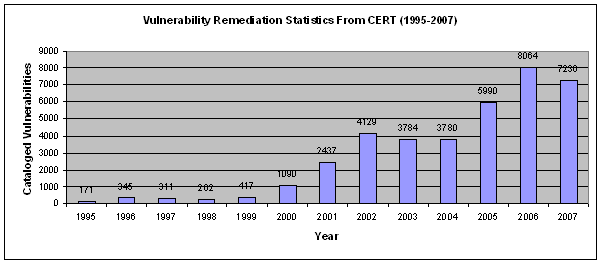
\includegraphics[width=0.8\textwidth]{Imgs/1.png}
    \caption{\label{fig:1} The Catalogued Vulnerabilities Data from CERT Coordination Center from 1995 to 2007  \cite{One}.}
\end{figure}
Due to its importance, researchers have proposed various approaches to defend against buffer overflow attacks. However, each of them has its own limitations and cannot be applied universally to prevent overflow attacks. 

In this project, it is aimed to detect and test buffer overflow vulnerabilities in a source code using static analysis techniques. \cite{Two}


\section{MOTIVATION}
Being able to detect overflows would improve software assurance. Static analysis can be used as a baseline for determining the susceptibility of a program to cause buffer overflows.  

When a new buffer overflow vulnerability is first exploited, a primary challenge is to diagnose the vulnerability. The diagnosis results include which buffer was overflowed; under what conditions the buffer will be overflowed. 

This research investigates the viability of a buffer overflow detection method to statically analyse source files for buffer overflows. The research focuses on the discovery of stack-based, heap-based and integer overflows that occur in C programs.